\chapter{マトロイド} \label{chap:matroid}
マトロイド(matroid)は「行列(matrix)のようなもの(-oid)」という名を冠するが,
ベクトルの線型独立性を拡張した独立性の概念として\citet{Whitney1935}によって定義された.

\section{定義}
\begin{definition}{マトロイド}{matroid}
    次の性質を持つ単体複体$(V,\F)$を\emph{マトロイド (matroid)}という:
    任意の$\sigma,\tau \in \F$に対し, $\abs{\sigma} < \abs{\tau}$ならば,
    ある$ u \in \tau \setminus \sigma$が存在して
    $\sigma \cup \cbra{u} \in \F$.

    マトロイド$(V,\F)$の面$\sigma\in \F$を特に\emph{独立集合 (independent set)}という.
\end{definition}

\begin{definition}{基}{basis}
    マトロイドの(包含関係に関して)極大な独立集合を\emph{基 (basis)}といい, 基全体の集合を$\B$で表す.
    特に断りのない限り, 基上の定常分布は一様分布とする.
\end{definition}
マトロイドは純粋な単体複体である.
実際, もし$\abs{B} < \abs{B'}$なる二つの基$B,B'\in\B$が存在するならば,
マトロイドの定義(\cref{def:matroid})より,
ある$u \in B'\setminus B$が存在して$B\cup \{u\} \in \F$とできるが,
これは$B$の極大性に矛盾する.

本講義ではマトロイドの基上の定常分布は常に一様分布とする.

\paragraph*{例1. 一様マトロイド}
\cref{eq:uniform matroid}で定まる単体複体$(V,\F)$は\emph{一様マトロイド (uniform matroid)}と呼ばれるマトロイドである.

\paragraph*{例2. グラフ的マトロイド}
\cref{eq:graphic matroid}で定まる単体複体$(V,\F)$はマトロイドである.
ここでは証明の概要を説明する.
マトロイドであることを示すには, 任意の二つの森$\sigma,\tau \in \F,\abs{\sigma} < \abs{\tau}$に対して, ある辺$e\in \tau\setminus \sigma$が存在して$\sigma\cup\{e\}$が閉路を含まないようにできることを言えばよい.
二つの森$\sigma,\tau \in \F,\abs{\sigma} < \abs{\tau}$を固定する.
森$\sigma\in \F$はグラフ上で複数の連結成分をなす.
これら連結成分の個数は$|V| - \abs{\sigma}$に等しい.
さて, 森$\tau$の中には, $\sigma$のなす連結成分のうち相異なる二つの間を横切る辺$e \in \tau \setminus \sigma$が存在する (\cref{fig:graphicmatroid}).
そうでなければ, $\tau$のなす連結成分の個数$|V|-\abs{\tau}$は$|V|-\abs{\sigma}$以下となってしまい, $\abs{\tau} > \abs{\sigma}$に矛盾.
この辺$e$を$\sigma$に追加しても閉路は発生しない.
(もし閉路$C$が生じるならば, $e$が$\sigma$のなす連結成分を横切ることに矛盾する).
すなわち, $\sigma\cup\{e\}\in\F$であり, 確かに$(V,\F)$はマトロイドである.
%
\begin{figure}
    \begin{center}
    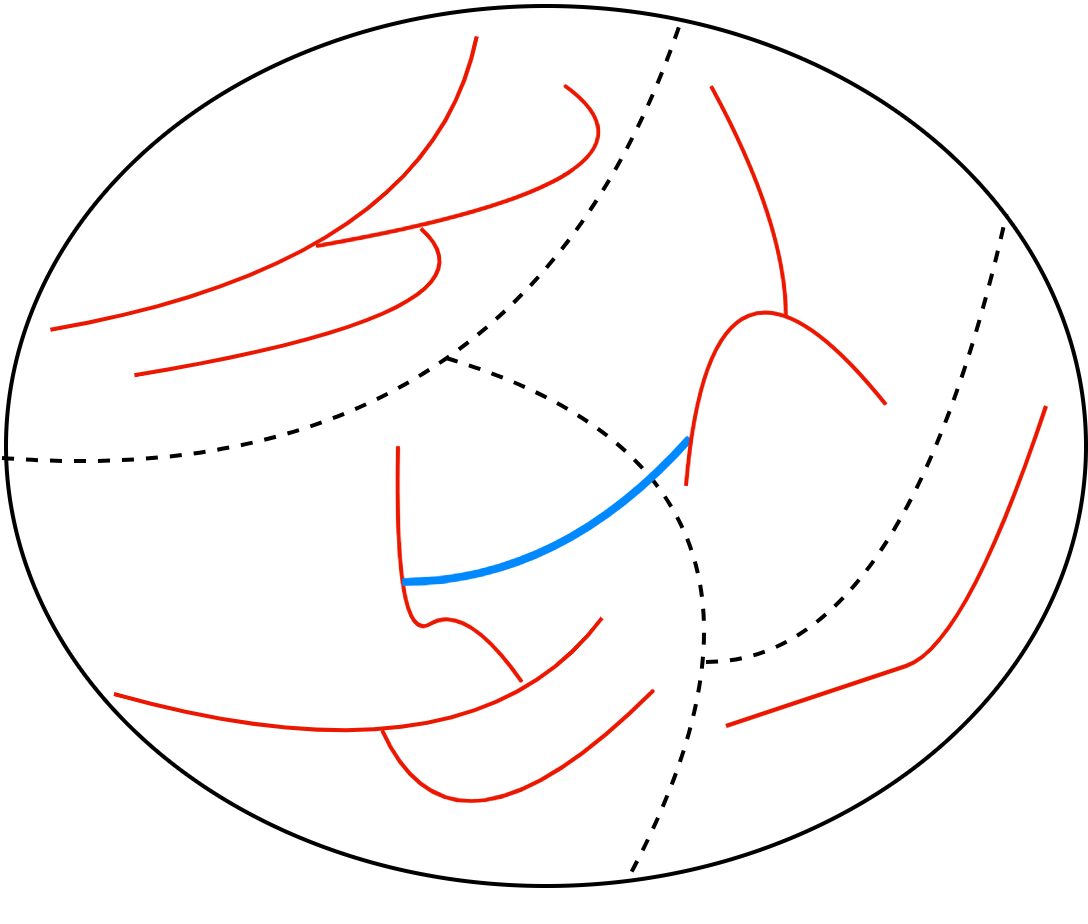
\includegraphics[width=7cm]{images/graphicmatroid.png}
    \caption{森$\sigma$のなす連結成分をまたがる辺$e \in \tau$が必ず存在する. \label{fig:graphicmatroid}}
    \end{center}
\end{figure}

グラフの森から定まる上記のマトロイドは\emph{グラフ的マトロイド (graphic matroid)}と呼ばれるマトロイドの重要なクラスをなす.

%
\paragraph*{例3. 線形マトロイド}
\cref{eq:linear matroid}で定まる単体複体$(V,\F)$は\emph{線形マトロイド (linear matroid)}と呼ばれるマトロイドである.
$\sigma,\tau\in \F$であって$\abs{\sigma} < \abs{\tau}$であるとする.
全てのベクトル$x\in \tau$が$x\in \mathrm{span}(\sigma)$に属するならば, $\tau$の線型独立性に矛盾するのであるベクトル$x\in \tau$が存在して$\{x\}\cup\sigma\in\F$となる.

\paragraph*{例4. 分割マトロイド}
有限集合$V$の分割$V=W_1\sqcup \dots \sqcup W_k$と非負整数$d_1,\dots,d_k\ge 0$を固定する.
部分集合族$\F$を
\begin{align}
    F \in \F \iff \forall i\in\{1,\dots,k\},\abs{W \cap W_i} \le d_i     \label{eq:partition matroid}
\end{align}
で定義したとき, $(V,\F)$は\emph{分割マトロイド (partition matroid)}と呼ばれるマトロイドである.
平たく言えば, 各$W_i$の元を高々$d_i$個ずつ含むものからなる部分集合族である.

\begin{exercise}{}{partition matroid}
    \cref{eq:partition matroid}で定まる単体複体$(V,\F)$がマトロイドであることを示せ.
\end{exercise}

\paragraph*{マトロイドでない例.}
クリーク複体やマッチング全体のなす単体複体はそもそも純粋とは限らないので必ずしもマトロイドになるとは限らない.

\section{基交換ウォーク}
\begin{definition}{基交換ウォーク}{basis-exchange walk}
    マトロイド$(V,\F)$の基上の下降上昇ウォークを\emph{基交換ウォーク (basis-exchange walk)}という.
\end{definition}
$X(d-1)$から$X(d)$への上昇ウォークを考えてみよう.
$\pi_{d-1}(\sigma)=\sum_{\tau\in\B} \pi_d(\tau) \cdot \Pdown_d(\tau,\sigma)$は, $\pi_d$が一様分布であり$\Pdown_d(\tau,\sigma)$は$\allone_{\tau\supset \sigma}$に比例するため, $\sigma$を含む基の個数に比例する.
従って
\begin{align*}
    \Pup_{d-1}(\sigma,\tau) = \frac{\pi_d(\tau)\Pdown_d(\tau,\sigma)}{\pi_{d-1}(\sigma)} \propto \allone_{\tau\supset \sigma}
\end{align*}
を得る.
すなわち, 基$B$から開始する基交換ウォークは,
一様ランダムに元$u\sim B$を選び,
$B\setminus u$を含む基の中から一様ランダムな基$B'\in B'$に遷移するランダムウォークであり, その定常分布は一様分布である.
基交換ウォークの混交時間のバウンドは長年の未解決問題であった.
\begin{conjecture}{Mihail--Vazirani予想}{Mihail-Vazirani}
    任意のマトロイド$M=(V,\F)$上の基交換ウォークの混交時間は$|V|$に関する多項式で上から抑えられる.
    すなわち, $M$に依存しないある定数$c>0$が存在して
    \[
        \tmix(1/2) \le |V|^c.
    \]
\end{conjecture}
基全体の個数は$\abs{V}$に関して指数関数的であるが,
ここでは
\emph{多項式ステップ}の基交換ウォークで混ざり合うかを問うている.
グラフ的マトロイドといった特殊ケースでは\cref{conj:Mihail-Vazirani}が正しいことが知られていた
\cite{balanced_matroids}が, 一般のマトロイドで正しいかどうかは未解決であった.

\section{マトロイドの局所エクスパンダー性}
本節では以下の定理を証明する.
\begin{lemma}{}{local expander matroid}
    任意のマトロイド$(V,\F)$は局所$0$-エクスパンダーである.
\end{lemma}


\subsection{Oppenheimのトリクルダウン定理}
ある単体複体$X$に対して局所エクスパンダー性(\cref{def:local expander})を示すには全ての面に対して$\lambda_2(P_\sigma)$を上から抑える必要がある.
一般にそもそも辺重み$w_\sigma$ (\cref{def:local random walk}) を求めることすら非自明であり, ましてや固有値を抑えるなど非常に大変な作業となる.
Oppenheimのトリクルダウン定理\cite{Oppenheim_tricling_down}は局所エクスパンダー性を確認するのに非常に有用な定理である.
\begin{theorem}{Oppenheimのトリクルダウン定理}{Oppenheim trickle-down theorem}
    純粋な重み付き$d$-次元単体複体$X = (V,\F)$が以下の二つを満たすとする:
    \begin{itemize}
    \item 全ての$i\le d-2$と全ての$\sigma\in X(i)$に対してグラフ$G_\sigma$は連結.
    \item 全ての$(d-2)$-次元の面$\tau \in X(d-2)$に対して$\lambda_2(P_\tau) \le \gamma$.
    \end{itemize}
    このとき, $\gamma_i \defeq \frac{\gamma}{1-(d-2-i)\gamma}$ ($i=-1,\dots,d-2$)に対して$X$は局所$(\gamma_{-1},\dots,\gamma_{d-2})$-エクスパンダーである.
\end{theorem}
端的に言えば, 次数$d-2$の面$\sigma \in X(d-2)$に対して$\lambda(P_\sigma)$を抑えれば全ての次元の面に対しても第二固有値が上から抑えられるという結果である.
最上次元の面のエクスパンダー性が下次元の面に波及していくという意味ではまさに「トリクルダウン(浸透)」といえよう.

一つ目のグラフ$G_\sigma$の連結性の条件は不可欠である.
例えば二つの完全グラフからなる非連結グラフ上の三角形複体を考えると,
空集合以外の全てのリンクは完全グラフ上のランダムウォークとなるため$\gamma=0$に対して二つ目の条件を満たすが, $\sigma=\emptyset$に対して$G_\sigma$は非連結であるため$\gamma_{-1}=0$にはならない.


\cref{thm:Oppenheim trickle-down theorem}は, まず$d=2$の特殊ケースで証明し, 一般の$d$についてはこの特殊ケースに帰着する.
%
\begin{lemma}{\texorpdfstring{$d=2$}{2次元}におけるトリクルダウン定理}{trickle-down for 2dim}
    純粋な重み付き$2$次元単体複体$X=(V,\F)$の各頂点$v\in X(0)$における局所ランダムウォーク$P_v$が$\lambda_2(P_v) \le \gamma$を満たし, かつその$1$-スケルトン$G_v$が連結ならば, 面$\emptyset$における局所ランダムウォーク$P_\emptyset$は
    \[
        \lambda_2(P_\emptyset) \le \frac{\gamma}{1-\gamma}
    \]
    を満たす.
\end{lemma}
この補題は本質的に$\gamma<1/2$のときに意味をなす.
\subsection{ランダムウォークの分解}
\cref{lem:trickle-down for 2dim}の証明は,
\cref{thm:Kaufman-Oppenheim theorem}と同様にランダムウォークを分解することから始まる.
記法の簡単のため, 頂点$u$のリンクを$X_{\{u\}}$の代わりに$X_u$, 遷移確率行列を$P_{\{u\}}$の代わりに$P_u$と表す.
\begin{definition}{}{localize}
    重み付き単体複体$(V,\F)$, 頂点$u\in V$, 関数$f \in \ispace[X(0)]$に対し,
    関数$f^u \in \ispace[X_u(0)]$を$f$の$X_u(0)$への制限, すなわち
    \[
        f^u (v) = f(v)
    \]
    とする.
\end{definition}
簡単な計算から以下の二次形式の分解補題が成り立つことがわかる.
\begin{lemma}{}{decomposition}
    任意の$f,g\in \ispace[X(0)]$に対して
    \[
        \iprod[X(0)]{f,g} = \E_{u\sim X(0)}\sbra*{ \iprod[X_u(0)]{f^u,g^u} }.
    \]
    また, 面$\emptyset$上の局所ランダムウォークの遷移確率行列を$P_\emptyset \in [0,1]^{X(0)\times X(0)}$とすると,
    \[
        \iprod[X(0)]{P_\emptyset f,g} = \E_{w\sim X(0)}\sbra*{ \iprod[X_u(0)]{P_uf^u,g^u} }.
    \]
\end{lemma}
\begin{proof}
    最初の等式を示す:
    \begin{align*}
        (\text{左辺}) &= \E_{u\sim X(0)} \sbra*{ f(u) g(u) } \\
        &= \E_{e \sim X(1)}\sbra*{ \E_{v \sim e} \sbra*{f(v)g(v)}} & & \text{$v\sim e$の周辺分布は$\pi_0$}\\
        &= \E_{u\sim X(0)} \sbra*{ \E_{\substack{e=\{u,v\} \sim X(1) \\ \text{conditioned on }e\ni u} }\sbra*{ f(v)g(v) }} & & \text{$e\sim X(1)$の$v$でない方の端点$u$を先に選ぶ}\\
        &= \E_{u\sim X(0)}\sbra*{ \E_{v \sim X_u(0)} \sbra*{f^u(v) g^u(v)} } & & \text{$\because$\cref{rem:link of u}}\\
        &= (\text{右辺}).
    \end{align*}
    二つ目の等式を示す.
    \begin{align*}
        (\text{左辺}) &= 
        \E_{\substack{u\sim X(0)\\ v\sim P_\emptyset(u,\cdot)}} \sbra*{ f(u)g(v)}\\
        &= \E_{t \sim X(2)}\sbra*{ \E_{\substack{w \sim t \\ u \sim t\setminus \{w\}, \\ \{v\}=t\setminus\{u,w\}}} \sbra*{f(u)g(v)} } \\
        &= \E_{w\sim X(0)}\sbra*{ \E_{\substack{t \sim X(2) \\ \text{conditioned on }t \ni w \\ u \sim t \setminus w \\ \{v\}=t\setminus\{u,w\}}} \sbra*{f(u)g(v)} } & & \text{前式の$w$の周辺分布は$X(0)$}\\
        &= \E_{w\sim X(0)}\sbra*{ \E_{\substack{u\sim X_w(0) \\ v\sim P_w(u,\cdot)}}\sbra*{f(u)g(v)} } \\
        &= (\text{右辺}).
    \end{align*}
\end{proof}
%
\begin{proof}[\textbf{\cref{lem:trickle-down for 2dim}の証明.}]
    記号の簡単のため$P=P_\emptyset$とする.
    局所ランダムウォーク$P$の第二固有値に対応する固有ベクトルを$f$とする.
    正規化して$\inorm[X(0)]{f}=1$とする.
    $P_\emptyset$の可逆性および\cref{lem:Rayleigh quotient}から,
    $\iprod[X(0)]{f,\allone}=0$である.
    補題を証明するには, $ \lambda_2(P)=\iprod[X(0)]{P f,f}$を上から抑えればよい.

    各頂点$u \in X(0)$に対し\cref{def:localize}で定義された$f^u \in \ispace[X_u(0)]$を考える.
    このベクトルを直交分解し,
    \begin{align}
        f^u = \alpha_u \allone^u + \overline{f^u} \label{eq:eigen decomposition fu}
    \end{align}
    と表す.
    ここで, $\allone^u \in \ispace[X_u(0)]$は全成分が$1$のベクトルで, $\alpha_u=\iprod[X_u(0)]{f,\allone^u}$であり, $\overline{f^u}$は$\allone^u$に直交するベクトルである.

    直交分解(\ref{eq:eigen decomposition fu})を用いると
    \begin{align*}
        \iprod[X_u(0)]{P_u f^u,f^u} &= \iprod[X_u(0)]{P_u\rbra*{\alpha_u\allone^u + \overline{f^u}}, \alpha_u\allone^u+\overline{f^u}} \\
        &= \iprod[X_u(0)]{\alpha_u \allone^u + P_u\overline{f^u}, \alpha_u\allone^u+\overline{f^u}} \\
        &= \alpha_u^2 + \iprod[X_u(0)]{P_u\overline{f^u},\overline{f^u}}  & & \text{直交性よりクロスタームは消える}\\
        &\le \alpha_u^2 + \gamma\inorm[X_u(0)]{\overline{f^u}}^2 & & \text{$\because$$\lambda_2(P_u)\le \gamma$および\cref{lem:Rayleigh quotient}}
    \end{align*}
    を得る.
    \cref{lem:decomposition}より,
    \begin{align*}
        \lambda_2(P) &= \iprod[X(0)]{Pf,f} \\
        &= \E_{u\sim X(0)}\sbra*{ \iprod[X_u(0)]{P_u f^u,f^u} } & & \text{$\because$\cref{lem:decomposition}の二つ目の等式} \\
        &\le \E_{u\sim X(0)}\sbra*{\alpha_u^2} + \gamma\cdot \E_{u\sim X(0)}\sbra*{\inorm[X_u(0)]{\overline{f^u}}^2} & & \text{直前の不等式を代入}\\
        &= \gamma\cdot \E_{u\sim X(0)}\sbra*{\alpha_u^2 + \inorm[X_u(0)]{\overline{f^u}}^2} + (1-\gamma)\cdot \E_{u\sim X(0)}\sbra*{\alpha_u^2} \\
        &= \gamma\cdot \E_{u\sim X(0)}\sbra*{\inorm[X_u(0)]{f^u}^2} + (1-\gamma)\cdot \E_{u\sim X(0)}\sbra*{\alpha_u^2} & & \text{$\because$$f^u$に対する三平方の定理}\\
        &= \gamma \cdot \inorm[X(0)]{f}^2 + (1-\gamma)\cdot \E_{u\sim X(0)}\sbra*{\alpha_u^2} & & \text{$\because$\cref{lem:decomposition}を$\iprod[X(0)]{f,f}$に適用} \\
        &= \gamma + (1-\gamma)\cdot \E_{u\sim X(0)}\sbra*{\alpha_u^2} & & \text{$f$のノルムは$1$}
    \end{align*}
    を得る.
    従って, $\E_{u\sim X(0)}\sbra*{\alpha_u^2}$を上から抑えたい.

    内積$\iprod[X_u(0)]{\cdot,\cdot}$の定義から
    \begin{align*}
        \alpha_u &= \iprod[X_u(0)]{f^u,\allone^u} \\
        &= \E_{v \sim X_u(0)}\sbra*{f^u(v)} \\
        &= \E_{v \sim X_u(0)}\sbra*{ f(v) } & & \text{\cref{def:localize}参照}\\
        &= (Pf)(u) & & \text{$P=P_\emptyset$は$1$-スケルトン上のランダムウォーク}
    \end{align*}
    であり, $f$は$P$の固有ベクトルなので
    \begin{align*}
        \E_{u\sim X(0)}\sbra*{\alpha_u^2} &= \inorm[X(0)]{Pf}^2 = \lambda_2(P)^2.
    \end{align*}
    これを代入すると二次不等式
    \begin{align*}
        \lambda_2(P) \le \gamma + (1-\gamma)\lambda_2(P)^2
    \end{align*}
    を得る. これを$\lambda_2(P)$について解くと
    \[
     \lambda_2(P)\ge 1 \text{ または }\lambda_2(P) \le \frac{\gamma}{1-\gamma}
    \]
    となるが, $1$-スケルトン$G_v$の連結性の仮定より$\lambda_2(P)<1$なので, $\lambda_2(P) \le \frac{\gamma}{1-\gamma}$を得る.    
\end{proof}
%
\subsection{トリクルダウン定理の証明}
\cref{lem:trickle-down for 2dim}を用いて一般の次元$d$に対する\cref{thm:Oppenheim trickle-down theorem}を証明する.
%
\begin{proof}[\textbf{\cref{thm:Oppenheim trickle-down theorem}の証明.}]
    $X=(V,\F)$を純粋な重み付き$d$次元単体複体とする ($d\ge 3$).
    面$\sigma \in X(d-3)$のリンク$X_\sigma$の次元は$2$であり,
    $X_\sigma$の頂点$v\in X_\sigma(0)$に対して
    $\sigma \cup \{v\} \in X(d-2)$より,
    $X_\sigma$上の$v$における局所ランダムウォークの遷移確率行列は$P_{\sigma\cup \{v\}}$に等しく, 仮定より$\lambda_2\rbra*{P_{\sigma\cup\{v\}}}\le \gamma$である.
    さらに, $X$の各リンクの$1$-スケルトンは連結なので, \cref{lem:trickle-down for 2dim}より
    \[
        \lambda_2(P_\sigma) \le \frac{\gamma}{1-\gamma}
    \]
    を得る.
    同じ議論を, $X$をその$(d-1)$-スケルトンに置き換えて適用すると,
    任意の$\sigma' \in X(d-4)$に対し
    \[
        \lambda_2(P_{\sigma'}) \le \frac{\frac{\gamma}{1-\gamma}}{1- \frac{\gamma}{1-\gamma}} = \frac{\gamma}{1-2\gamma}
    \]
    を得る.
    これを繰り返すと, ($j$に関する帰納法により)
    面$\rho \in X(d-2-j)$に対し
    \[
        \lambda_2(P_\rho) \le \frac{\gamma}{1-j\gamma}
    \]
    を得る.
\end{proof}
%


\section{Anari, Liu, Gharan, Vinzantの定理}
\begin{theorem}{Anari-Liu-Gharan-Vinzantの定理}{ALGV}
    任意のマトロイドは,
    \[ \lambda_i = 1-\frac{1}{i+1}\]
    に対して大域$(\lambda_0,\dots,\lambda_d)$-エクスパンダーである.
\end{theorem}
\begin{proof}
    次元$d$のマトロイド$X=(V,\F)$の独立集合$\sigma \in X(d-2)$を任意に固定し, リンク$X_\sigma$の$1$-スケルトン$G_\sigma$を考える.
    基$\B$上の定常分布は一様分布なので,
    $\sigma$に関する局所ランダムウォークは$G_\sigma$上の単純ランダムウォークとなる.
    さて, $G_\sigma$の頂点集合$V_\sigma$は
    \[V_\sigma = \{v\in V\setminus\sigma\colon \sigma\cup \{v\} \in \F\}\]
    であり,
    辺集合$E_\sigma \subseteq \binom{V_\sigma}{2}$は,
    \[
        E_\sigma = \cbra*{ \{u,v\}\colon \sigma\cup\{u,v\}\in \F }
    \]
    となる.

    ここで, 以下の命題を証明する:
    \begin{align}
        \{u,v\},\{v,w\}\not\in E_\sigma \Rightarrow \{u,w\} \not\in E_\sigma \label{eq:hogurahu clique}        
    \end{align}
    これは言い換えると$G_\sigma$の補グラフの全ての連結成分はクリークであることを意味する.
    命題(\ref{eq:hogurahu clique})を背理法で証明する.
    ある$\{u,v\},\{v,w\}\not\in E_\sigma$が存在して, さらに$\{u,w\}\in E$が成り立つと仮定する.
    このとき, $\tau\defeq \sigma\cup\{u,w\}\in \F$である.
    さらに, $v$は$G_\sigma$の頂点なので$\tau'\defeq \sigma\cup\{v\} \in \F$である.
    すなわち, $\tau,\tau'$は$\abs{\tau'} < \abs{\tau}$を満たす二つの独立集合なので, マトロイドの定義より
    ある$t \in \tau \setminus \tau' = \{u,w\}$に対して$\tau'\cup \{t\}=\sigma\cup\{u,t\} \in \F$, すなわち$\{u,t\}\in E_\sigma$となるが, これは$\{u,v\},\{v,w\}\not\in E$に矛盾する.

    主張(\ref{eq:hogurahu clique})より$G_\sigma$の補グラフの全ての連結成分はクリークである.
    これらを$C_1,\dots,C_\ell \subseteq V_\sigma$とし,
    $v_i\in \Real^{V_\sigma}$をクリーク$C_i$の指示ベクトルとする.
    $J\in\Real^{V_\sigma\times V_\sigma}$を全成分が$1$の行列とすると,
    $G_\sigma$の隣接行列$A\in\Real^{V_\sigma\times V_\sigma}$は
    \[
        A = J - \sum_{i=1}^\ell v_i v_i^\top
    \]
    となる.
    さらに, 局所ランダムウォークの定常分布$\pi^\sigma_0$を対角に並べた対角行列を$\Pi$とすると, 遷移確率行列は$P_\sigma = \Pi A = \Pi J - \sum_{i=1}^\ell \Pi v_iv_i^\top$となる.
    従って, 任意の$\iprod[V_\sigma]{f,\allone}=0$を満たす$f\in \ispace[V_\sigma]$に対して
    \begin{align*}
        \iprod[V_\sigma]{f,P_\sigma f} &= \iprod[V_\sigma]{f,\Pi J f} - \sum_{i=1}^\ell \iprod[V_\sigma]{f,\Pi v_iv_i^\top f} \\
        &= - \sum_{i=1}^\ell \iprod[V_\sigma]{f,\Pi v_iv_i^\top f} & & \text{$\because J f = 0$} \\
        &\le 0.
    \end{align*}
    最後の不等式では行列$\Pi v_iv_i^\top$が半正定値性を使った.
    これは,
    $\Pi v_i v_i^\top$がランク$1$行列であるため第二以降の固有値は全て$0$に等しく,
    さらに第一固有値はそのトレース$\mathrm{tr}(\Pi v_i v_i^\top) = \sum_{u\in V_\sigma} \pi^\sigma_0(u) v_i(u)^2\ge 0$に等しいことから従う.
    
    また, 全ての独立集合$\sigma\in \F$に対してリンク$X_\sigma$の$1$-スケルトン$G_\sigma$は連結である (演習問題).

    以上より, \cref{thm:thm:Oppenheim trickle-down theorem}からマトロイド$X$は局所$0$-エクスパンダーであり, さらに$\gamma=0$として\cref{thm:Kaufman-Oppenheim theorem}を適用すると主張を得る.
\end{proof}

\begin{exercise}{}{matroid connectivity}
    任意のマトロイド$X = (V,\F)$の任意の独立集合$\sigma \in \F$に対し,
    リンク$X_\sigma$の$1$-スケルトン$G_\sigma$は連結であることを示せ.
\end{exercise}

\begin{corollary}{マトロイド上のランダムウォークの混交時間}{}
    次元$d$の任意のマトロイド$(V,\F)$上の基交換ウォークの混交時間は
    \[
        \tmix(\varepsilon) = (d+1)|V|\log\rbra*{\frac{1}{\varepsilon}}.
    \]
    特に, \cref{conj:Mihail-Vazirani}は真である.
\end{corollary}
\begin{proof}
    \cref{thm:ALGV}および$\PDU_d$の半正定値性より$\lambda(\PDU_d) \le 1-\frac{1}{d+1}$ であり, $\PDU_d$のスペクトルギャップ(\cref{def:second eigenvalue})は少なくとも$\frac{1}{d+1}$である.
    また, 基上の定常分布$\pi=\pi_d$は基上の一様分布であり, 特に$\pimin \ge 1/2^{|V|}$が成り立つので, \cref{lem:mixing time and spectral gap}より, 
    \[
        \tmix(\varepsilon) \le \frac{\log\rbra*{\frac{1}{2\pimin\varepsilon}}}{\log(1/\lambda(P))} \le (d+1)|V|\log\rbra*{\frac{1}{\varepsilon}}.
    \]
\end{proof}